\documentclass[11pt,aspectratio=169,handout]{beamer}

\usetheme{Singapore}
\usecolortheme{orchid}

\usepackage[utf8]{inputenc}
\usepackage[russian]{babel}
\usepackage{amsmath}
\usepackage{amsfonts}
\usepackage{amssymb}
\usepackage{graphicx}
\usepackage{bibentry}
\usepackage{wasysym}
\usepackage[most]{tcolorbox}
\usepackage[normalem]{ulem}

\usepackage{hyperref}

\definecolor{info}{RGB}{62, 180, 137}
\definecolor{warn}{RGB}{1, 0, 0}

\author{Николай Анохин}
\title{Нерешенные проблемы и новые направления}

\logo{
\includegraphics[width=.05\textwidth]{images/ok_logo.png}}

\AtBeginSection[]{
  \begin{frame}
  \vfill
  \centering
  \begin{beamercolorbox}[sep=8pt,center,shadow=true,rounded=true]{title}
    \usebeamerfont{title}\insertsectionhead\par
  \end{beamercolorbox}
  \vfill
  \end{frame}
}

\begin{document}

{
\setbeamertemplate{headline}{}

\begin{frame}
\titlepage
\end{frame}

%\begin{frame}
%\tableofcontents
%\end{frame}

}

\begin{frame}{Контекст}

\begin{center}
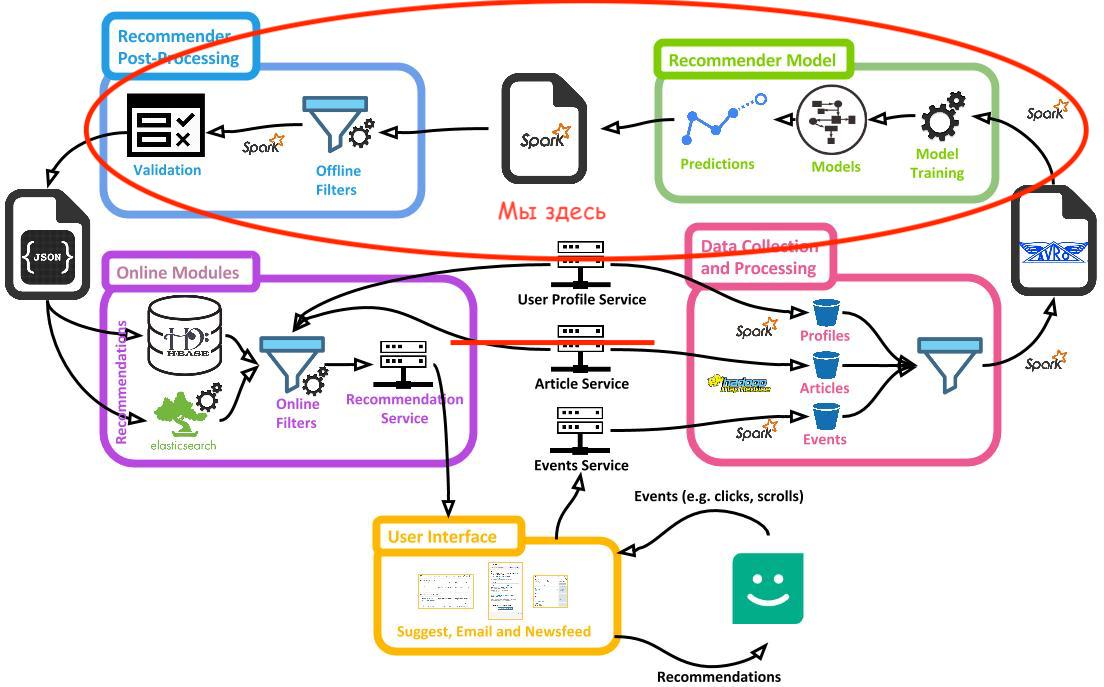
\includegraphics[scale=0.23]{images/mendeley.jpeg}
\end{center}

\end{frame}

\begin{frame}{Что мы уже умеем}

\begin{columns}

\begin{column}{0.55\textwidth}
\begin{center}
\begin{tcolorbox}[colback=info!5,colframe=info!80,title=]
\begin{large}
\[
\hat r_{ui} = f_{\theta}(x_u, x_i, x_c)
\]
\end{large}
\end{tcolorbox}\end{center}
\end{column}

\begin{column}{0.35\textwidth} 
\begin{center}

\includegraphics[scale=0.4]{images/simple.jpeg}
\end{center}
\end{column}
\end{columns}

\vfill

Проблемы
\begin{enumerate}[<+->]
\item {\color{blue} Оцениваем айтемы по-отдельности, а показываем по несколько (лентой)}
\item Смещение между распределениями на обучении и применении
\item Модель не объясняет, почему именно эти айтемы подходят пользователю
\item Не учитывается долгострочный эффект рекомендаций
\end{enumerate}

\end{frame}

\section{Разнообразие в рекомендательных системах}

\begin{frame}{Разнообразие / Diversity}

\begin{center}
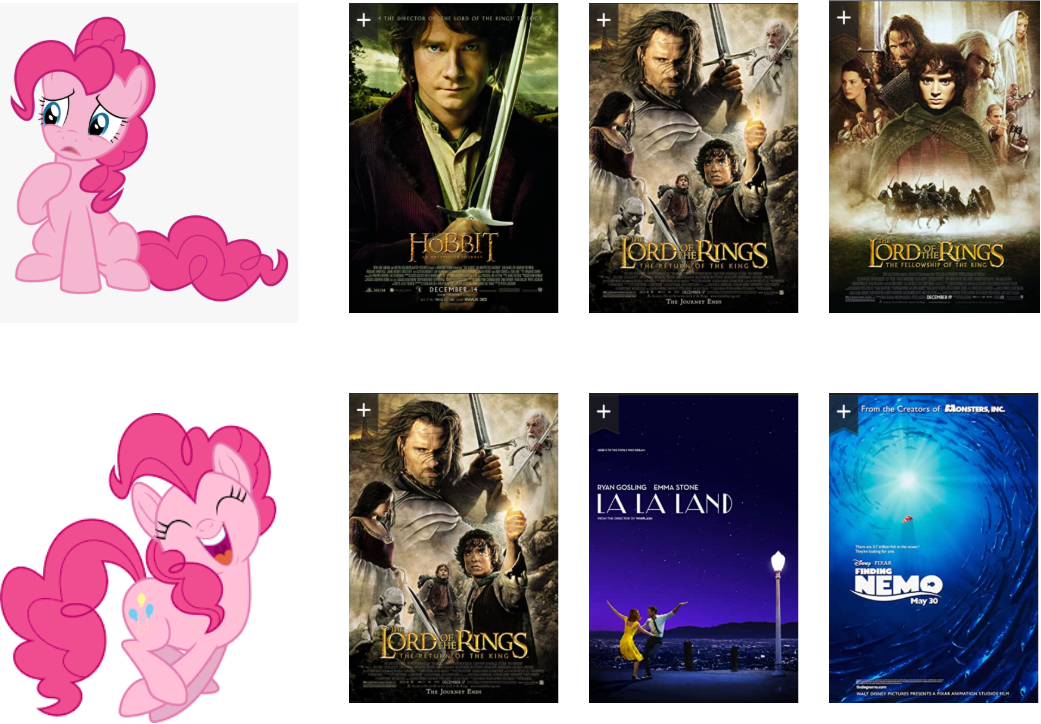
\includegraphics[scale=0.22]{images/diversity.png}
\end{center}

\end{frame}

\section{Разнообразие для exploration}

\begin{frame}{Разнообразие для exploration}

\begin{columns}

\begin{column}{0.55\textwidth}

Помогает
\begin{itemize}
\item пользователям находить новые айтемы
\item рекомендеру собирать данные
\end{itemize}

\end{column}

\begin{column}{0.35\textwidth} 
\begin{center}

\includegraphics[scale=0.2]{images/brian.png}
\end{center}
\end{column}
\end{columns}

\end{frame}

\begin{frame}{Набираем айтемы с разными аспектами}

$f$ - аспект (признак) айтема, $p(f | i)$ -- вероятность найти аспект у айтема $i$

\vfill

Распределение аспекта у пользователя

\[
p(f | u) = \frac{\sum_{i \in I_u} p(f | i)}{|I_u|}  
\]

Распределение аспекта в рекомендациях
\[
q(f | u) = \frac{\sum_{i \in RL} p(f | i)}{|RL|}
\]

\begin{tcolorbox}[colback=info!5,colframe=info!80,title=]
Формируем список так, чтобы $q(f | u)$ совпало с $p(f | u)$
\end{tcolorbox}

\end{frame}

\begin{frame}{Жадное переранжирование}

\begin{tcolorbox}[colback=info!5,colframe=info!80,title=]
Добавляем в список рекомендаций айтем с максимальным значением
\[
(1 - \lambda) \cdot s(u, i) + \lambda \cdot gain(i, RL),
\]
пока не получим список нужной длины.
\end{tcolorbox}

\vfill

\begin{itemize}
\item $s(u, i)$ -- релевантность айтема $i$ для пользователя $u$ 
\item $gain(i, RL) = div(RL \cup \{i\}) - div(RL)$ -- улучшение разнообразия при добавлении айтема
\item $\lambda$ -- гиперпараметр
\end{itemize}

\end{frame}

\begin{frame}{Примеры жадного переранжирования}

Maximal Marginal Relevance \cite{MMR}
\[
MMR = \arg \max_{D_i \in R \textbackslash S} \left[\lambda \cdot sim(D_i, Q) - (1 - \lambda) \cdot max_{D_j \in S} sim(D_i, D_j) \right].
\]
% SIGIR 98 - Tested on 5 students 80% chose MMR!

Mean Listing Relevance \cite{AIRBNB}
\[
MLR = \sum_{i=1}^N \left[ (1 - \lambda) \cdot c(i) P(l_i) + \lambda \sum_{j < i} \frac{d(l_i, l_j)}{i} \right],
\]
где $c(i)$ -- штраф за позицию в выдаче.

\end{frame}

\begin{frame}{Учим разнообразие вместе с моделью}

\begin{center}
Controllable Multi-Interest Framework for Recommendation \cite{ALIBABA}\footnote{Еще один подход к выученному разнообразию \cite{GENERATIVE}}
\end{center}

\begin{columns}
\begin{column}{0.45\textwidth}
\begin{center}
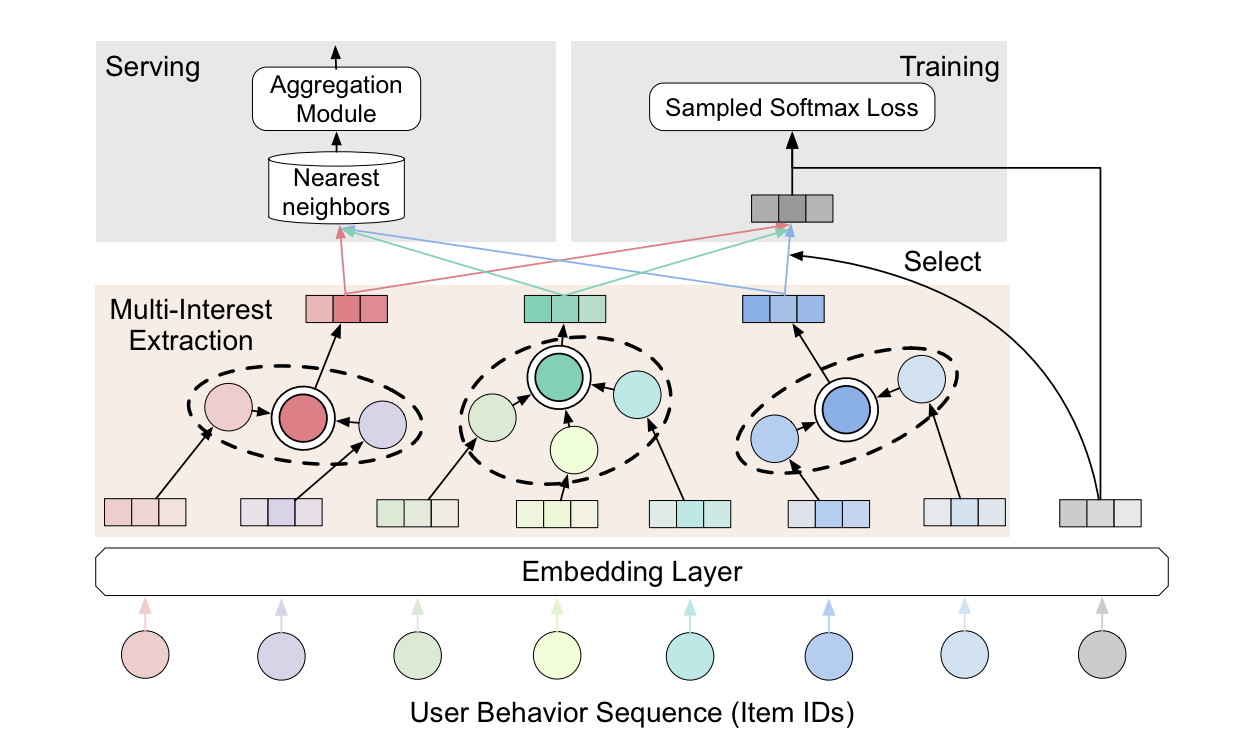
\includegraphics[scale=0.3]{images/alibaba.png}
\end{center}
\end{column}

\begin{column}{0.45\textwidth} 
\begin{center}
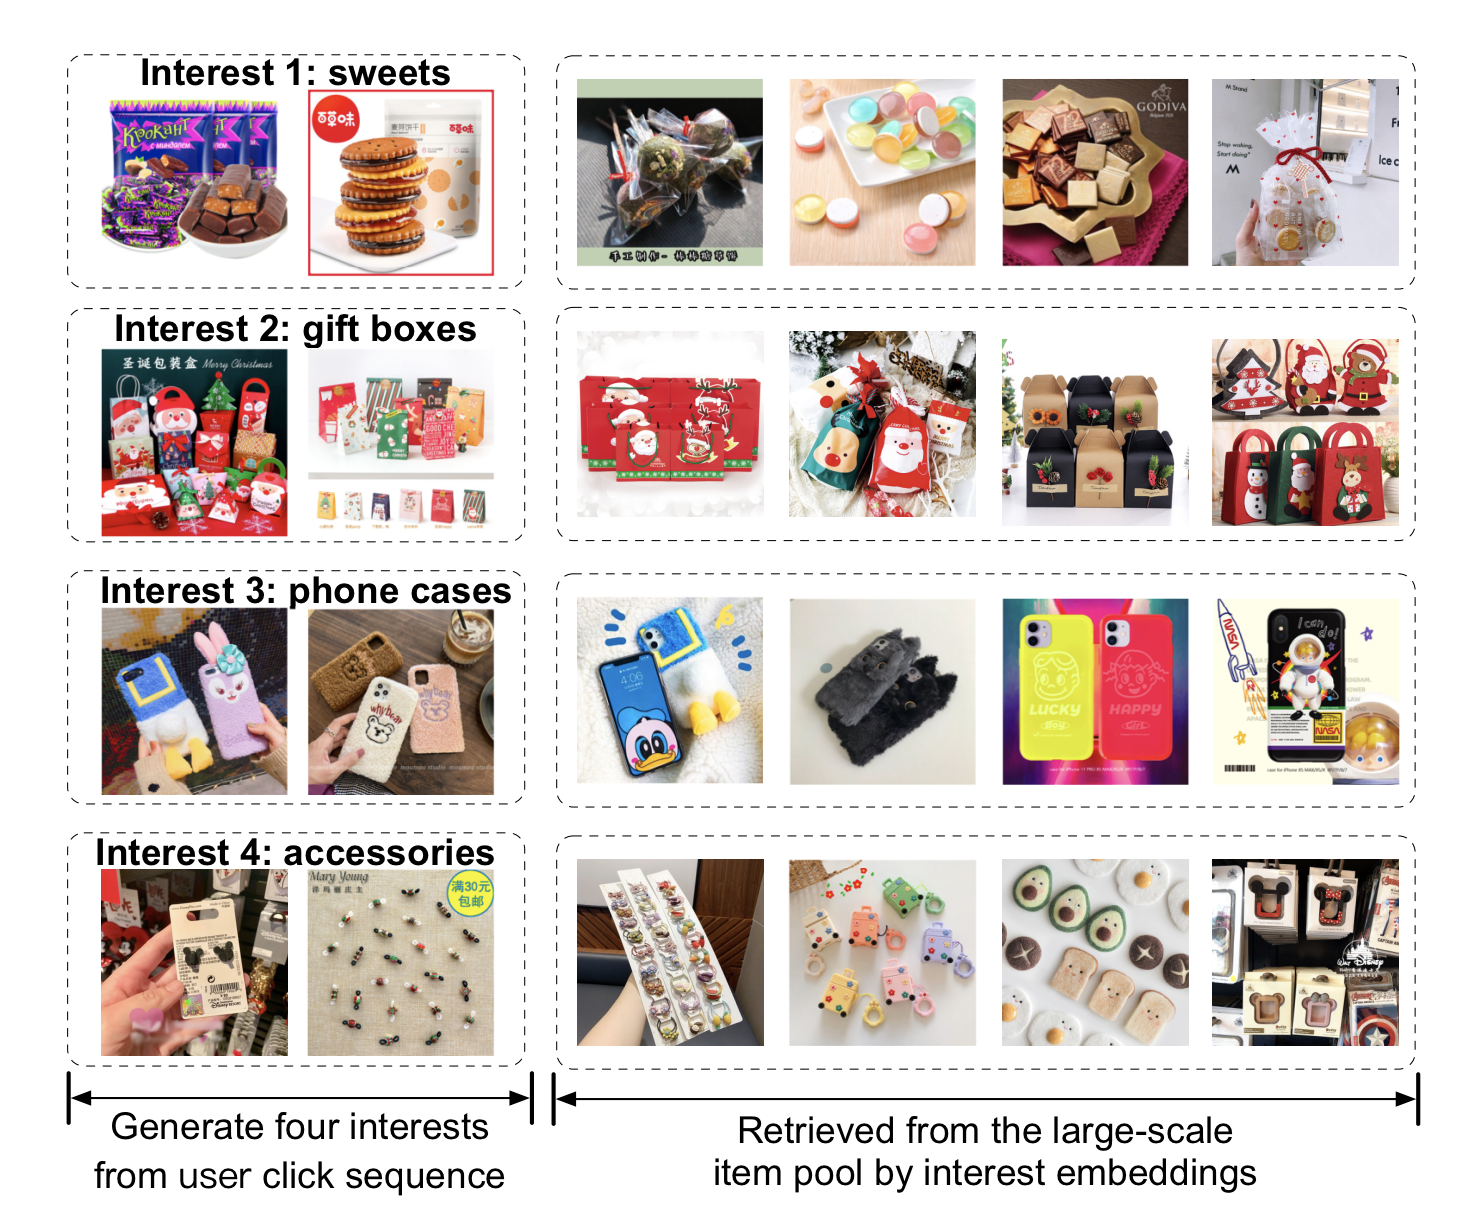
\includegraphics[scale=0.2]{images/divres.png}
\end{center}
\end{column}
\end{columns}

\end{frame}

\begin{frame}{A Comparison of Calibrated and Intent-Aware Recommendations \cite{BRIDGE}}
\begin{center}
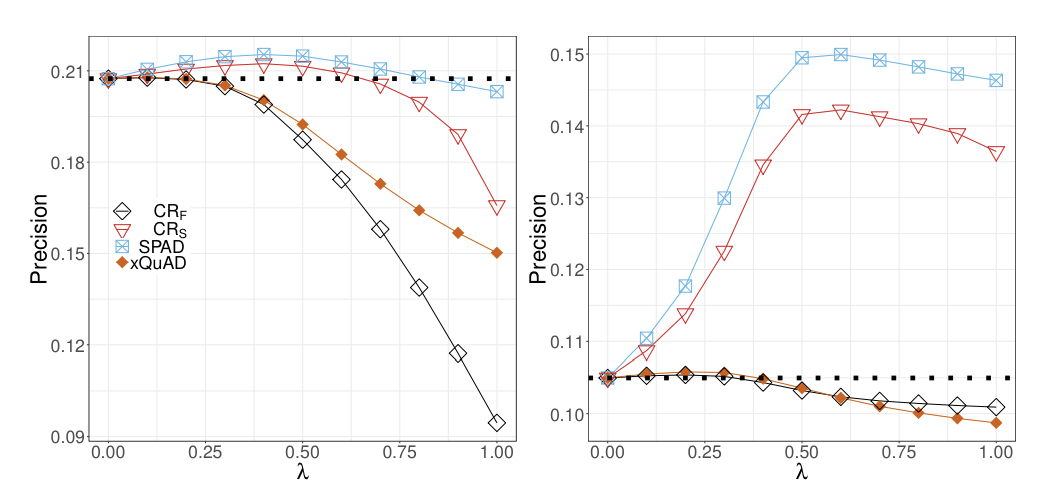
\includegraphics[scale=0.5]{images/spad.png}
\end{center}
\end{frame}

\begin{frame}

\begin{tcolorbox}[colback=info!5,colframe=info!80,title=]
Увеличивая разнообразие, мы готовы жертвовать (сиюминутной) релевантностью. Верим, что это принесет долгосрочный выигрыш.
\end{tcolorbox}

\end{frame}

\section{Разнообразие для utility}

\begin{frame}{Разнообразие для utility}

\begin{columns}

\begin{column}{0.45\textwidth}
Помогает
\begin{itemize}
\item убирать избыточные айтемы.
\end{itemize}
\end{column}

\begin{column}{0.45\textwidth} 
\begin{center}

\includegraphics[scale=0.2]{images/champ.png}
\end{center}
\end{column}

\end{columns}

\vfill

\begin{tcolorbox}[colback=info!5,colframe=info!80,title=]
При этом подходе компромисс relevance-diversity не существует!
\end{tcolorbox}

\end{frame}

\begin{frame}{Determinantal Point Process (DPP) \cite{DDP}}

Дано множество айтемов $S = \{1, 2, \ldots, N\}$.

\vfill

{\bf Point Process на S} -- распределение, определяющее вероятность $P(s)$ любого подмножества $s \subset S$.

\vfill

DPP (в рекомендациях) – это PP, в котором $P(s)$ тюнится так, чтобы бОльшая вероятность была у подмножеств с релевантными и разнообразными айтемами.

\end{frame}

\begin{frame}{Determinantal Point Process (DPP) contd.}

Пусть в рекомендательной выдаче $N$ айтемов, проиндексированных $\{1,\ldots, N\}$.

\vfill

$Y$ – множество индексов айтемов, с которыми было положительное взаимодействие (пример: $Y = \{2, 6, 11\}$).

\[
P(Y) = \frac{\det(L_Y)}{\sum_{Y'} \det(L_{Y'})}
\]

\end{frame}

\begin{frame}{Determinantal Point Process (DPP) contd.}

\begin{columns}

\begin{column}{0.45\textwidth}

$L$ – неотрицательно определенная матрица $N \times N$, в которой:
\begin{itemize}
\item диагональные элементы отвечают за релевантность
\item недиагональные – за попарное сходство.
\end{itemize}

\[
L_{ij} = f(q_i)^T g(\phi_i)^T g(\phi_i) f(q_i)
\]

\end{column}

\begin{column}{0.45\textwidth} 
\begin{center}
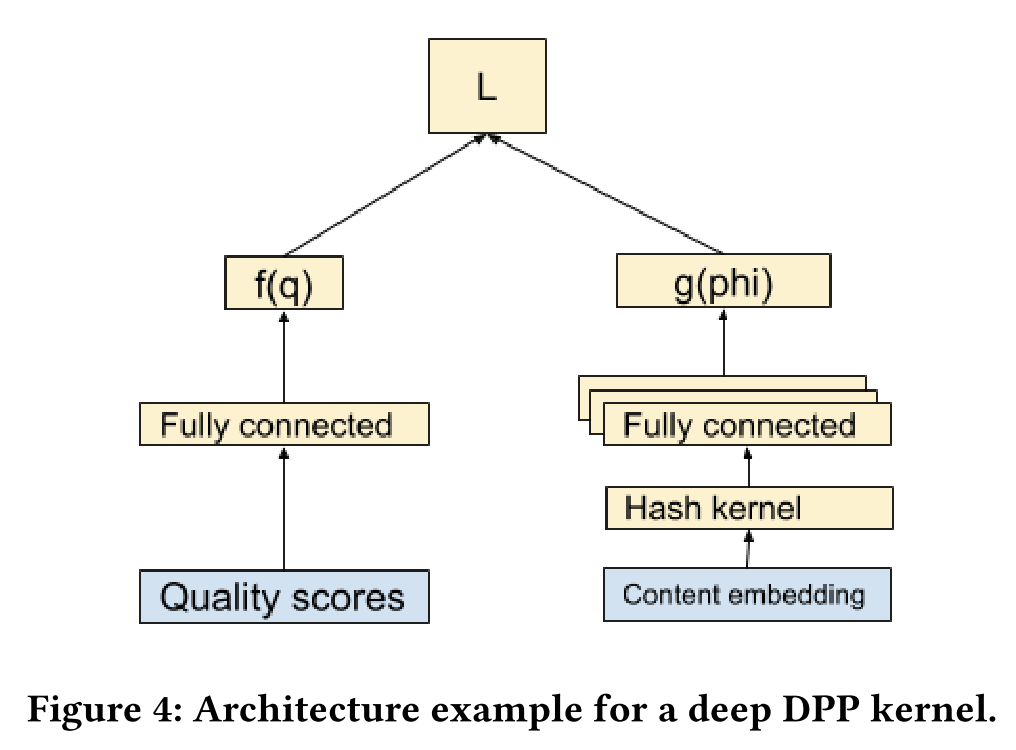
\includegraphics[scale=0.3]{images/dpp.png}
\end{center}
\end{column}

\end{columns}

\end{frame}

\begin{frame}{Determinantal Point Process (DPP) end.}

\begin{columns}

\begin{column}{0.45\textwidth}
{\bf Алгоритм}

На каждом шаге добавляем к $Y$ 
\[
\max_{v \not \subset Y} \det(L_Y \cup v),
\]
учитывая только последние $K$ айтемов.
\end{column}

\begin{column}{0.45\textwidth} 
\begin{center}
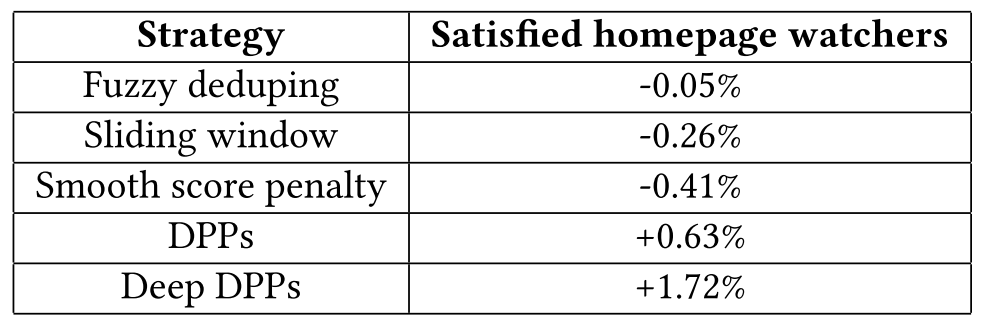
\includegraphics[scale=0.3]{images/ddp-res.png}
\end{center}
\end{column}

\end{columns}

\end{frame}

\begin{frame}{Managing Diversity in Airbnb Search \cite{AIRBNB}}

Идея: включить информацию, необходимую для разнообразия в модель, чтобы модель сразу выучила разнообразные рекомендации.\footnote{В \cite{AIRBNB2} эта модель сделана менее гибкой с помощью дополнительных предположений}

\begin{columns}

\begin{column}{0.45\textwidth}
\begin{center}
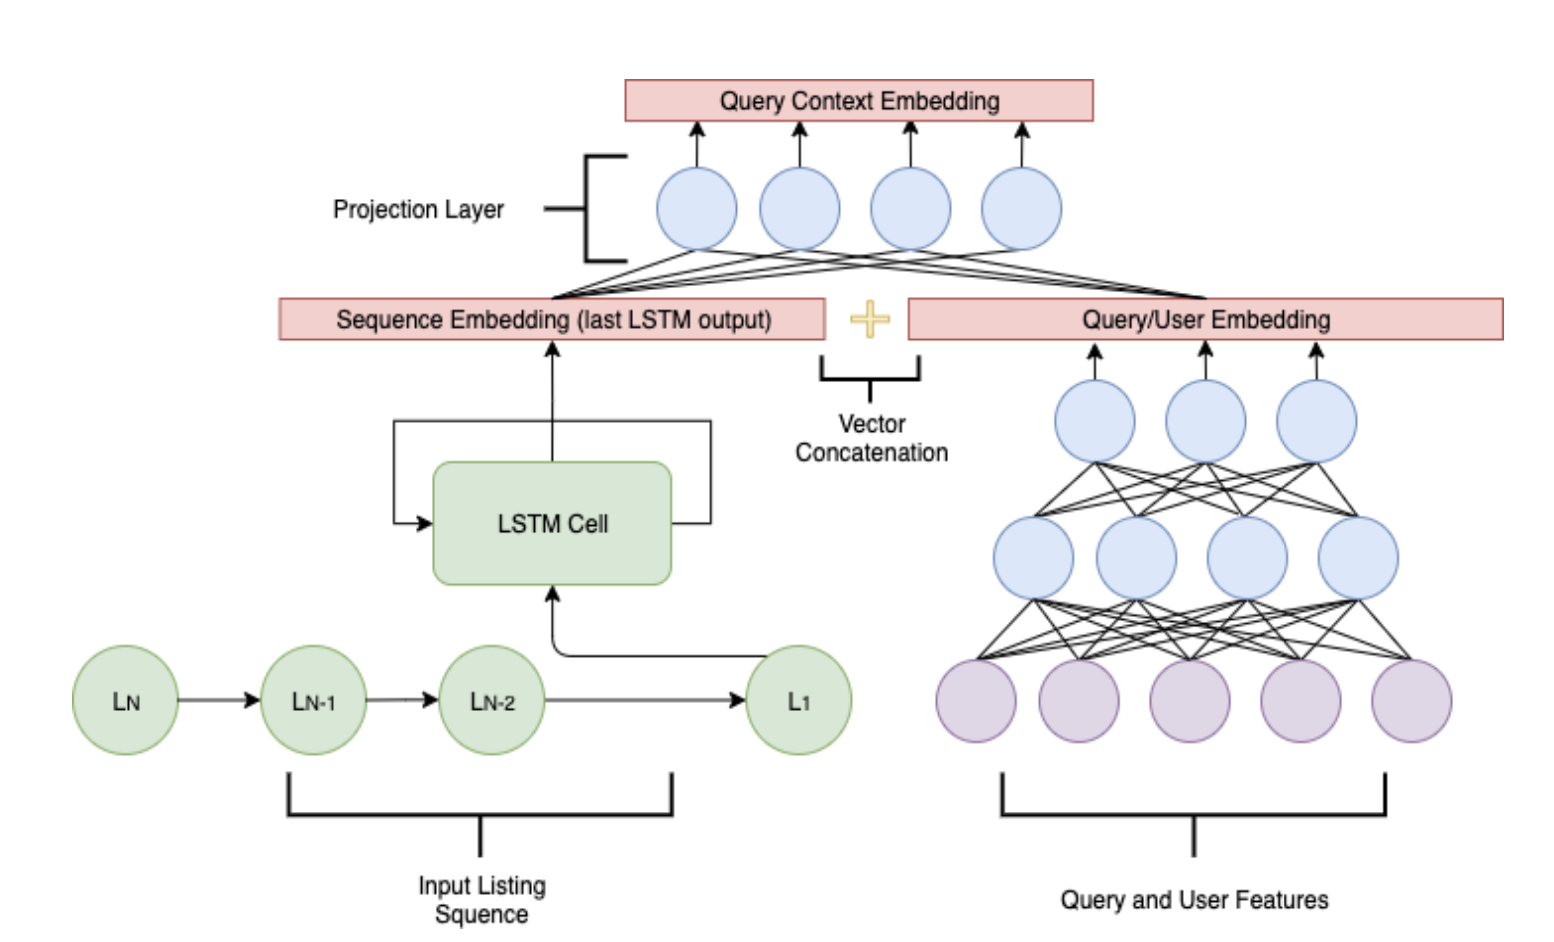
\includegraphics[scale=0.2]{images/airbnb2.png}
\end{center}
\end{column}

\begin{column}{0.45\textwidth} 
\begin{center}
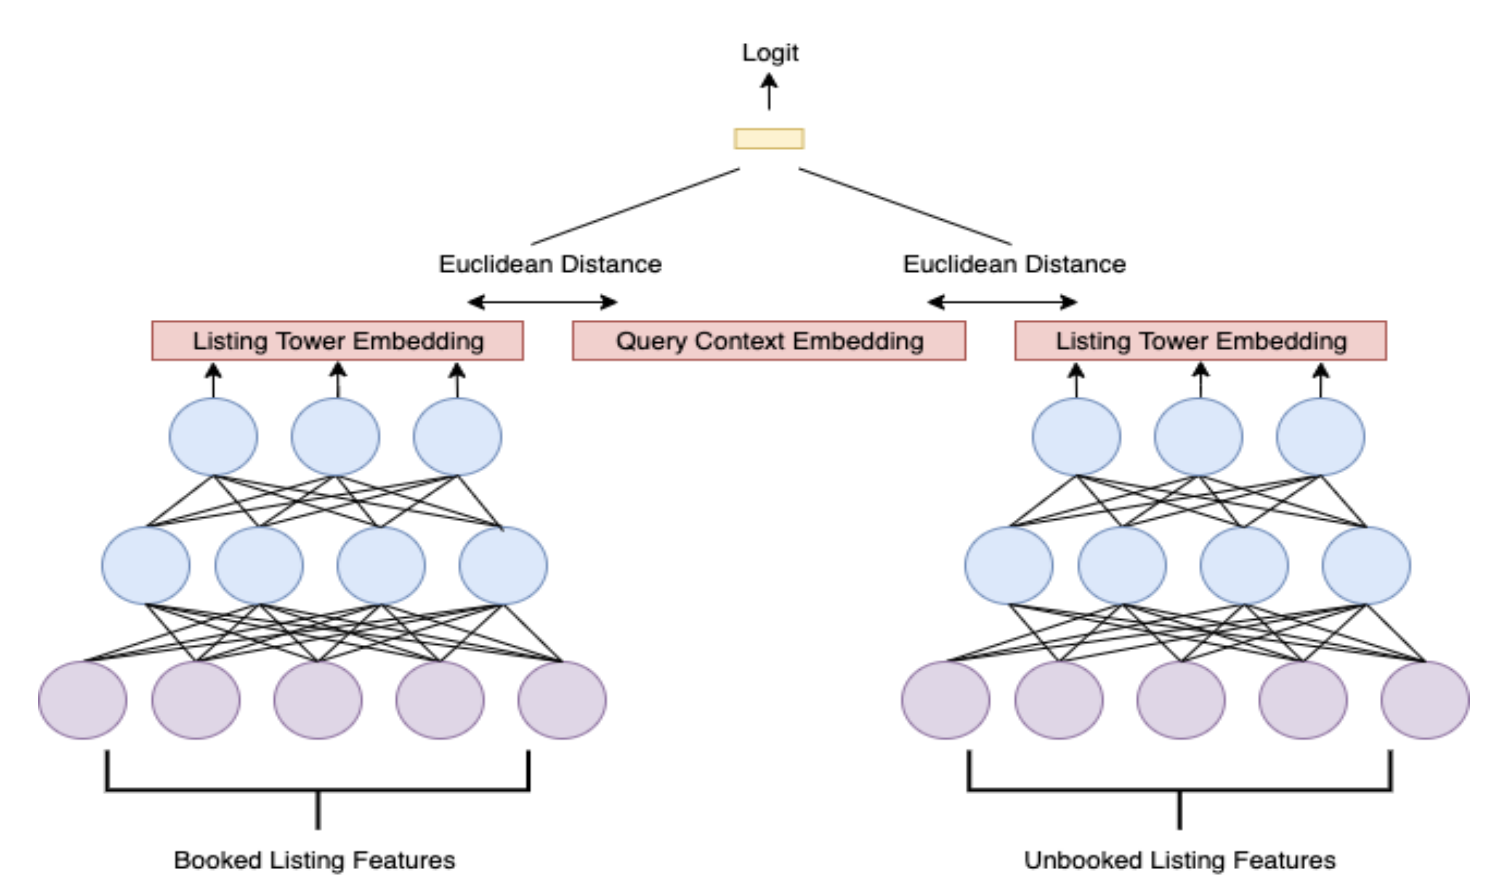
\includegraphics[scale=0.2]{images/airbnb.png}
\end{center}
\end{column}

\end{columns}

\begin{center}
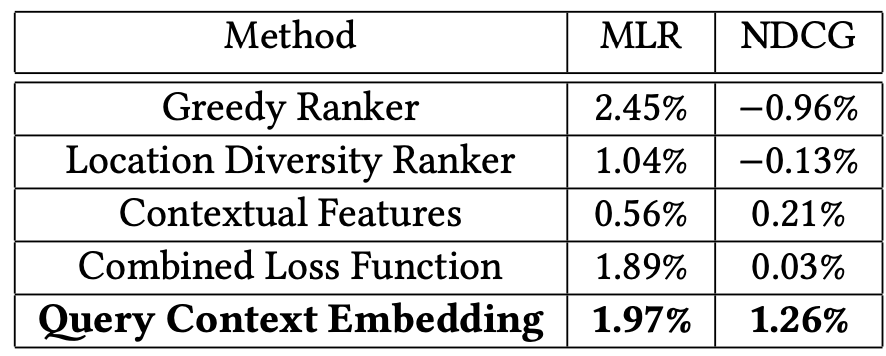
\includegraphics[scale=0.2]{images/airbnb-res.png}
\end{center}

\end{frame}

\begin{frame}

\begin{tcolorbox}[colback=info!5,colframe=info!80,title=]
Разнообразие можно рассматривать, как избавление от избыточности. Но для этого понадобятся модели построения списков.
\end{tcolorbox}

\end{frame}

\section{Итоги}

\begin{frame}{Итоги}

\begin{tcolorbox}[colback=info!5,colframe=info!80,title=]
Из-за поточечного предсказания релевантности, приходится дополнительно разнообразить списки рекомендаций
\end{tcolorbox}

\begin{tcolorbox}[colback=info!5,colframe=info!80,title=]
Можно смотреть на разнообразие как на exporation, но при этом быть готовым пожертвовать релевантностью.
\end{tcolorbox}

\begin{tcolorbox}[colback=info!5,colframe=info!80,title=]
Или можно смотреть на разнообразие как на избавление от избыточности, но это добавляет сложность при построении списков.
\end{tcolorbox}

\begin{tcolorbox}[colback=info!5,colframe=info!80,title=]
В любом случае, необходимость разнообразия можно обосновать A/B экспериментом.
\end{tcolorbox}

\end{frame}

\begin{frame}{}

\begin{columns}
\begin{column}{0.45\textwidth}
   \begin{center}
                
\includegraphics[scale=0.35]{images/bye.jpeg}
   \end{center}
\end{column}
\begin{column}{0.45\textwidth}
   \begin{center}
                \url{https://t.me/mlvok}

                
\includegraphics[scale=0.5]{images/tgqr.png}
   \end{center}
\end{column}
\end{columns}

\end{frame}

\begin{frame}[allowframebreaks]{Литература}

\bibliographystyle{amsalpha}
\bibliography{references.bib}

\end{frame}

\end{document}
